\subsubsection{General Considerations}
The Matrix Element method relies on the evaluation of the event probability densities for the signal and background processes based on the 
standard model differential cross-section calculation. 

In general, a differential cross-section is given by \cite{ref:PDG}:
\begin{equation}
d\sigma=\frac{(2\pi)^{4} \left| M \right|^{2}}{4\sqrt{(q_{1}q_{2})^{2}-m_{q_{1}}^{2}m_{q_{2}}^{2}}}d\Phi_{n}(q_{1}+q_{2};p_{1},...p_{n}),
\label{eqn:DiffXsecGeneral}  
\end{equation}
where $\left| M \right|$ is the Lorentz invariant matrix element;
$q_{1}$,$q_{2}$ and $m_{q_{1}}$,$m_{q_{2}}$ are the four momenta and masses of the incident particles 
(in our case quarks or gluons), 
$p_i$ is the four momentum of the $i-$th outgoing particle, 
and $d\Phi_{n}$ is the $n$-body phase space given by:
\begin{equation}
d\Phi_{n}(q_{1}+q_{2};p_{1},...p_{n})=\delta^{4}(q_{1}+q_{2}-\sum_{i=1}^{n}{p_{i}})\prod\frac{d^{3}p_{i}}{(2\pi)^{3}2E_{i}}.
\label{eqn:PhaseSpaceGeneral}  
\end{equation}
where the sum runs over the $n$ outgoing particles produced in the collision.
It is important to note here that energies of the incident partons are not known and are distributed according to the parton density 
functions (PDFs). Therefore, for a certain set of observed kinematic properties $x$, one can write the probability of observing it as:
\begin{equation}
P(x)=\frac{1}{\sigma}\int d\sigma(y)dq_{1}dq_{2}f(y_{1})f(y_{2})W(x;y),
\label{eqn:EvtProbGeneral}  
\end{equation}
where $y=(p_{1}...p_{n})$ is the set of parton level variables needed to describe an event, $d\sigma(y)$ is the differential cross-section 
in terms of $y$, $f(y_{1})$ and $f(y_{2})$ are the PDFs and $W(x;y)$ is a transfer function which maps parton level quantities to the 
reconstructed quantities.  One can think of $W(x;y)$ as the probability of observing a reconstructed event $x$ given an event with parton level properties $y$. $\sigma$ is a normalization constant which is discussed separately below.

Assuming that  the momenta of the incident partons have no transverse component, the four vectors can be written as:
\begin{equation}
q_{1}=(0,0,\xi_{1}E_{beam},\xi_{1}E_{beam}),
q_{2}=(0,0,-\xi_{2}E_{beam},\xi_{2}E_{beam}),
\label{eqn:EvtProbGeneral2}  
\end{equation}
where $\xi_{1}$ and $\xi_{2}$ are fractions of the proton energy carried by the initial partons as given by the PDFs, and
$E_{beam}=3.5$ TeV. Assuming that the initial state partons are massles, we can rewrite the ``flux'' term:
\begin{equation}
\frac{1}{\sqrt{(q_{1}q_{2})^{2}-m_{q_{1}}^{2}m_{q_{2}}^{2}}} \approx \frac{1}{2 E_{q_{1}}E_{q_{2}}}.
\label{eqn:flux}  
\end{equation}
where $E_{q_{i}} = \xi_i\times E_{beam}$.  
Taking into account Eq.~\ref{eqn:DiffXsecGeneral} and \ref{eqn:PhaseSpaceGeneral}, and considering final states with four particles,
Eq.~\ref{eqn:EvtProbGeneral} can be re-written as:
\begin{equation}
P(x)=\frac{1}{ \sigma}\int 2 \pi^{4} \left| M \right|^{2} \frac{f(y_{1})f(y_{2})}{(E_{q_{1}}E_{q_{2}})^{2}}W(x;y)d\Phi_{4}dE_{q_{1}}dE_{q_{2}},
\label{eqn:EvtProbGeneral3}  
\end{equation}
or
\begin{equation}
P(x)=\frac{1}{\sigma }\int 2 \pi^{4} \left| M \right|^{2} \frac{f(\xi_{1})f(\xi_{2})}{\xi_{1}\xi_{2}E_{beam}^{2}}W(x;y)d\Phi_{4}d\xi_{1}d\xi_{2},
\label{eqn:EvtProbGeneral4}  
\end{equation}

\subsubsection{Normalization Constant}
If the integration is performed over the entire kinematic phase space, then the normalization term $\sigma$ is equal
to the total cross-section $\sigma_{total}$.  However, if the integration is performed only over the acceptance region,
then $\sigma=A\sigma_{total}$, where $A$ is the acceptance term for a given physics process, or in other words the fraction
of the total cross-section falling into the acceptance region.  The acceptance term $A$ can be derived as:
\begin{equation}
A=\frac{N_{accepted}}{\sigma_{total}\times L},
\label{eqn:Acceptance}  
\end{equation}
where $N_{accepted}$ is the expected yield of events passing the acceptance selection, and $L$ is the integrated luminosity.

\subsubsection{Effect of the system boost}
Equation \ref{eqn:EvtProbGeneral3} is derived assuming no transverse component of the momenta of the incident partons,
which is true at Leading Order.   At next-to-leading order (NLO), however, initial state radiation (ISR) can generate a transverse momentum
of the system.  The distribution of the system transverse momentum depends on the amount of ISR and its $p_{T}$ spectrum, and
therefore may vary for different physics processes. In the presence of a transverse boost, the general probability expression can
be rewritten as:
\begin{equation}
P(x)=\frac{1}{\sigma }\int 2 \pi^{4} \left| M \right|^{2} \frac{f(\xi_{1})f(\xi_{2})}{\xi_{1}\xi_{2}E_{beam}^{2}}\epsilon(y)G(x;y)d\Phi_{4}d\xi_{1}d\xi_{2}K(k_{x},k_{y})dk_{x}dk_{y},
\label{eqn:EvtProbGeneralWithBoost}  
\end{equation}
where $K(k_{x},k_{y})$ is the transverse momentum distribution and $W(x;y)=\epsilon(y)G(x;y)$ is factorized into a reconstruction 
efficiency term $\epsilon(y)$ and a resolution function $G(x,y)$ accounting for detector resolution effects.
The efficiency and transfer functions are described in more detail in Sec.~\ref{sec:EfficiencyTransfer}.

\subsubsection{$l^{+}l^{-}\nu\bar{\nu}$ final state }
For the Higgs to $WW$ leptonic final state, $H \rightarrow WW \rightarrow l^{+}l^{-}\nu\bar{\nu}$, assuming no jet activity, 
the set of reconstructed quantities can be written as $x=(\vec{p}_{l1},\vec{p}_{l2}, \met_{x},  \met_{y})$.
The complication of this state is that it is not fully reconstructed, and information about the $z$-components of the neutrino 
momenta as well as individual neutrino transverse components are missing. It is, therefore, necessary to integrate over these 
unknown quantities. Expression \ref{eqn:EvtProbGeneralWithBoost} for this case can be written as:
\begin{eqnarray}
P(x)=\frac{1}{\sigma }\int 2 \pi^{4} \left| M \right|^{2} \frac{f(\xi_{1})f(\xi_{2})}{\xi_{1}\xi_{2}E_{beam}^{2}}
\epsilon(\vec{p}_{l1})\epsilon(\vec{p}_{l1}) \times \nonumber \\ 
                         G(p_{l1},p_{l2}, \met_{x},  \met_{y}; q_{l1}, q_{l2}, p_{\nu_{1,x}}+  p_{\nu_{2,x}}, p_{\nu_{1,y}}+p_{\nu_{2,y}})d\Phi_{4}d\xi_{1}d\xi_{2} \times \nonumber \\
                         K(k_{x},k_{y})dk_{x}dk_{y}\delta(p_{\nu_{1,x}}+p_{\nu_{2,x}}-\met_{x})\delta(p_{\nu_{1,y}}+p_{\nu_{2,y}}-\met_{y}).
\label{eqn:EvtProbGeneralWithBoost2L2nu}  
\end{eqnarray}
where $q_{l1}$ and $q_{l2}$ are true momenta of the leptons.

\subsection{Evaluation of the Differential Cross-Section}

\subsubsection{Integration}
The evaluation of the differential cross section requires integration over the missing kinematic information in an event, such 
as the longitudinal components of neutrino momenta, as well as integration over allowed values of the transverse momentum
of the system.

We perform the integration using Monte Carlo techniques, in which we generate values of unknown quantities based on a set of
random numbers.  Monte Carlo calculations can be carried out using sets of random points picked from any arbitrary probability 
distribution. The choice of the underlying distribution obviously makes a difference to the efficiency of the method. In most cases,
Monte Carlo calculations carried out using uniform probability distributions give very poor estimates of high-dimensional integrals
and are not a useful method of approximation. 
Therefore, we employ the algorithm of ``importance sampling'' in the Monte Carlo integration. Instead of choosing points from a 
uniform distribution, they are chosen from a distribution which concentrates the points in the region of phase space where the 
value of the function being integrated is large.  For example,
\begin{equation}
\label{eqn:ImpSampling}
I=\int_{x_{1}}^{x_{2}} f(x)dx = \int_{a}^{b} \frac{f(x)}{g(x)}dx,
\end{equation}
where the function $g(x)$ is chosen to be a reasonable approximation to $f(x)$. The integral can be calculated by choosing the random points 
from the probability distribution $g(x)$ and evaluating $f(x)/g(x)$ at these points.  Sampling from a non-uniform distribution for this function 
is more efficient than doing a crude Monte Carlo calculation without importance sampling.

The number of integration variables depends on the process for which the differential cross-section is evaluated. For example,
in the case of the gluon fusion signal there are four missing components of the neutrino momenta,
$(\nu_{x}, \nu_{y}, \nu_{z}, \bar{\nu}_{z})$, after including the $x$ and $y$~components of the $\met$.  
These quantities, in addition to the measured ones and also the two components of the transverse boost 
($k_{x}$ and $k_{y}$), fully define the system.
However, integration using  $(\nu_{x}, \nu_{y}, \nu_{z}, \bar{\nu}_{z})$ as the set of variables is not efficient.  Due to the narrow 
Breit-Wigner width of the Higgs and $W$ bosons, most points chosen at random from a uniform distribution will lie outside of 
the core of the cross-section function. To avoid this and improve the
efficiency of the integration, we perform the variable transformations 
$\nu_{x} \rightarrow m_{H}^{2}$ and $\nu_{y} \rightarrow m_{W}^{2}$ 
so that the set of integration variables becomes $(m_{H}^{2}, m_{W}^{2}, \nu_{z}, \bar{\nu}_{z})$.
A Jacobian corresponding to the transformation is calculated analytically and properly 
accounted for. The integration is then performed using the importance sampling method, with neutrino $z$-components sampled
using an exponential function and $m_{H}^{2}$ and $m_{W}^{2}$ using narrow Breit-Wigner distributions.
Similarly, for non-resonant $WW$ production, the set of variables used for the integration is:
$(m_{W1}^{2}, m_{W2}^{2}, \nu_{z}, \bar{\nu}_{z})$. In the $W$+jet case, there is only one missing quantity $\nu_{z}$ which is sampled using 
an exponentially falling function.

For each event we perform 100,000 integration steps. To verify that this is sufficient, for randomly selected events we calculate differential cross
sections using 500,000 integration steps and compare them to the ones obtained with 100,000. In the vast majority of cases the difference
was $< 1\%$ and the largest observed deviation was $\sim 5\%$. 

\subsubsection{Comparison of Differential Cross Section for Signal and Background Events}

Integration over the event-by-event differential cross-section $\frac{d\sigma}{dx}$ is used to evaluate the probability $P$ as described
in Equation~\ref{eqn:EvtProbGeneral}.  Since we expect to see different probabilities for signal and background events,
we should see separation in the differential cross-sections for different signal and
background processes when looking at the same events.  For now we restrict our comparison to just the signal,
$H\rightarrow WW$, and the dominant background, non-resonant $WW$ production.

Figure~\ref{subfig:HWWXsec} shows the differential cross section for gluon fusion Higgs production,
$d\sigma(H \rightarrow WW)/dx$, calculated for gluon fusion Higgs signal events and for non-resonant $WW$ events.
The distribution for signal events is shifted to larger values of  $d\sigma(H \rightarrow WW)/dx$ compared to that
of non-resonant $WW$, and it has a narrower width. 
Figure~\ref{subfig:HWWXsecvsdPhi} shows the distribution of $d\sigma(H \rightarrow WW)/dx$ as a function of
$\Delta\phi_{ll}$ for signal and non-resonant $WW$ events.
As described in Sec.~\ref{sec:Meth_Overview}, the distributions of $\Delta\phi_{ll}$ are different for the signal and the $WW$
background due to spin effects. We see here that the differential cross-section is correlated with $\Delta\phi_{ll}$ and is on average decreasing with
increasing azimuthal angle, since the signal will be concentrated at smaller values of $\Delta\phi_{ll}$.
Figure~\ref{subfig:Xsec_WWvsHWW} shows distributions of these events in the $d\sigma(H \rightarrow WW)/dx$ 
vs. $d\sigma(WW)/dx$ plane. One can see that while a certain level of separation can be achieved, there is a 
non-negligible overlapping region of phase space where events from the two processes are indistinguishable.
%Finally, figure~\ref{subfig:to be inserted} shows distributions of signal and $W$+jet 
%events in $d\sigma(H \rightarrow WW)/dx$ vs $d\sigma(W+jet)/dx$ plane (this one needs to be made and inserted).

\begin{figure}[!hbtp]                                                                                         
\centering                                                                                                    
\subfigure[]{                                                                                                 
\centering                                                                                                    
\label{subfig:HWWXsec}                                                                                       
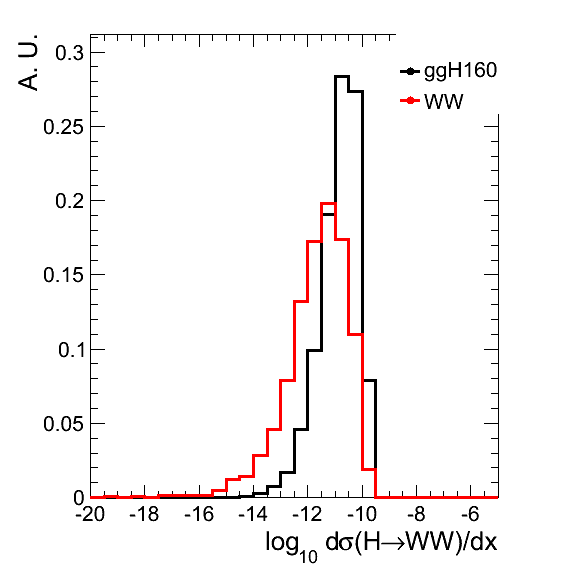
\includegraphics[width=.42\textwidth]{figures/HWWXsec.png}}                                                                                       
\subfigure[]{                                                                                                 
\centering                                                                                                    
\label{subfig:HWWXsecvsdPhi}                                                                                       
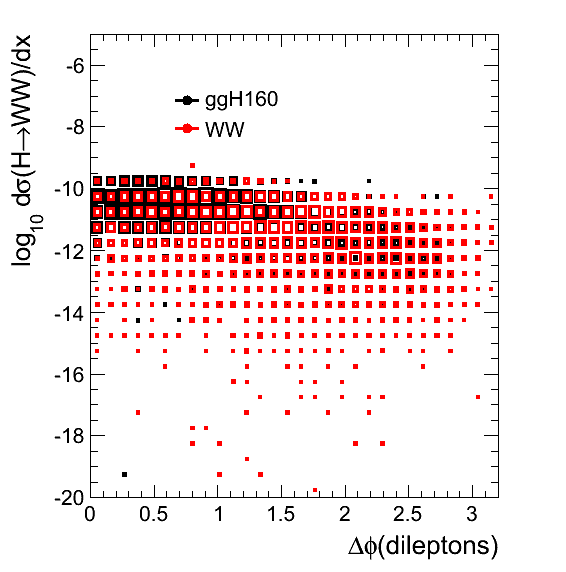
\includegraphics[width=.42\textwidth]{figures/HWWXsecvsdPhi.png}}                                            
\subfigure[]{                                                                                                 
\centering                                                                                                    
\label{subfig:Xsec_WWvsHWW}                                                                                       
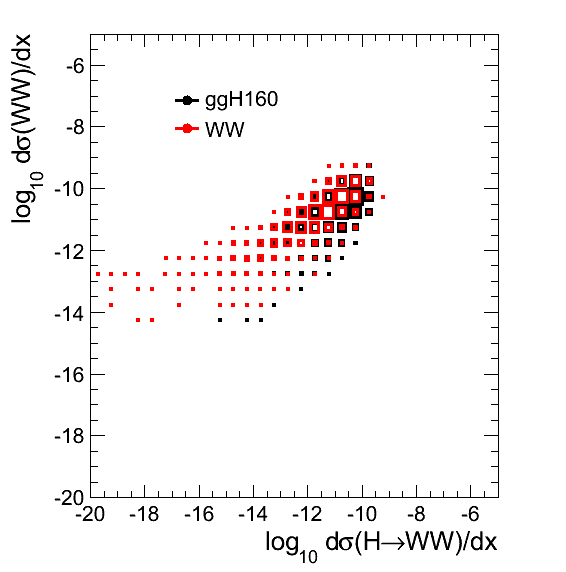
\includegraphics[width=.42\textwidth]{figures/Xsec_WWvsHWW.png}}\\                                            
\caption{Distributions of \subref{subfig:HWWXsec} the differential cross-section, $d\sigma(H \rightarrow WW)/dx$, 
\subref{subfig:HWWXsecvsdPhi} differential cross-section vs. $\Delta\phi_{ll}$, and 
\subref{subfig:Xsec_WWvsHWW}  $d\sigma(H \rightarrow WW)/dx$ vs. $d\sigma(WW)/dx$, 
for simulated Higgs signal and non-resonant $WW$ events.}
\label{fig:dXsecPlots}                                                                                          
\end{figure}                      

\subsubsection{$k_{T}$ Functions} 
In the leading order Matrix Element calculation there is no initial state radiation. The initial state partons 
collide head-on and the system has no transverse boost. To account for the transverse recoil and thus improve the performance 
of our discriminant on data, we integrate over the possible values of the system boost $K(k_x,k_y)$. The $K(k_x,k_y)$ model
is extracted from Monte Carlo for each process separately. Figure~\ref{fig:wwboost} shows a comparison of the distributions
of transverse boost for gluon fusion Higgs production at three different values of $m_H$ and the 
non-resonant $W^{+}W^{-}$ process.

\begin{figure}[!htbp]                                                                                         
\begin{center}                                                                                                
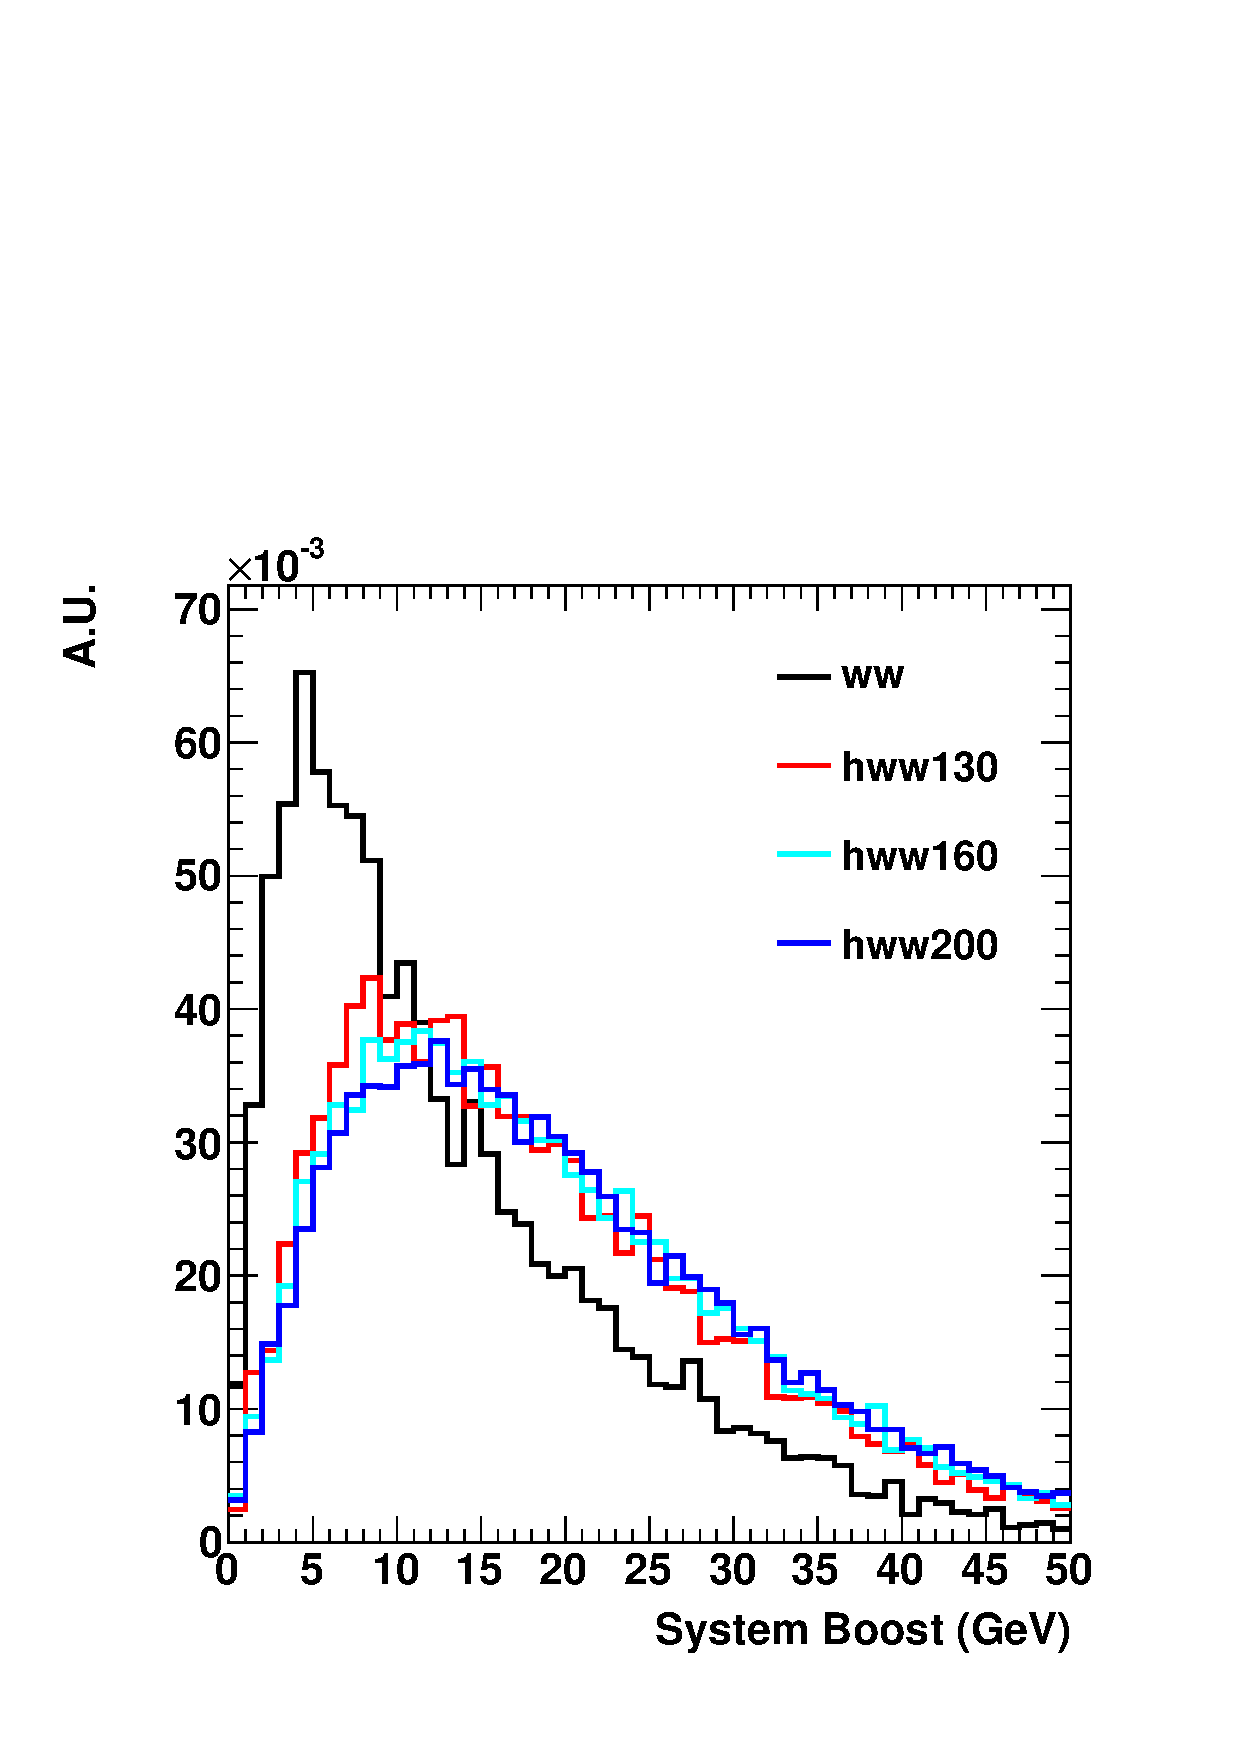
\includegraphics[width=0.5\textwidth]{figures/boost.pdf}                                                      
\caption{The transverse boost of the $WW$ system for $WW$ production and $H \rightarrow WW$ at 3 different Higgs masses.} 
\label{fig:wwboost}                                                                                           
\end{center}                                                                                                  
\end{figure}    

The effect of accounting for the transverse boost of the $WW$ system in the calculations of the differential cross-section
is demonstrated in Figure~\ref{fig:kteffect}. In the absence of the boost, there is a tail in the differential cross-section distribution
for Higgs signal events, with some events having small values of $d\sigma(H \rightarrow WW)/dx$.  
These events would likely be classified as background-like. Accounting for the system boost removes this tail,
allowing for better signal and background discrimination. 

\begin{figure}[!hbtp]                                                                                         
\centering                                                                                                                                             
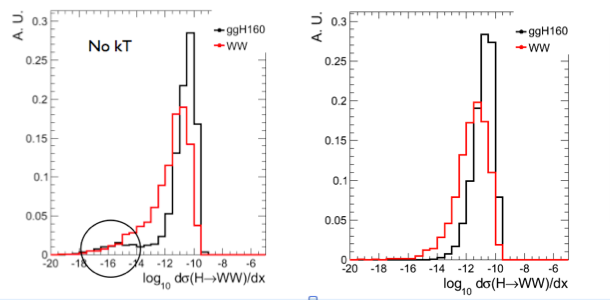
\includegraphics[width=.84\textwidth]{figures/SystemBoostEffect.png}\\                                            
\caption{
Distributions of the differential cross-section, $d\sigma(H \rightarrow WW)/dx$ for simulated Higgs signal and non-resonant $WW$ events
(a)using no system boost $K$, and (b) including a system boost.}
\label{fig:kteffect}                                                                                          
\end{figure}          

\subsection{Probability Calculations and Likelihood Ratio}
\label{sec:Probability}
The evaluation of the event probability was described in Sec.~\ref{sec:Evt_Prob} and 
Eq.~\ref{eqn:EvtProbGeneralWithBoost}~and~\ref{eqn:EvtProbGeneralWithBoost2L2nu}.
Two components of the determination of the event probability are the efficiency
and transfer functions described in detail here.

\subsubsection{Efficiency and Transfer Functions}
\label{sec:EfficiencyTransfer}
The efficiency functions $\epsilon(\vec{p})$ provide the probability that a lepton of given momentum
will be reconstructed in the detector. We evaluate this probability using non-resonant $q\bar{q}\rightarrow WW$
separately for muons and electrons and parametrize the probability as a function of the reconstructed
lepton $p_{T}$ and $\eta$.
The probability in each ($p_{T}$,$\eta$) bin is defined as the number of fully reconstructed leptons divided 
by the number of generator level leptons. Figure~\ref{fig:lepeff_gen} shows the 
one dimensional projection of the efficiency as a function of the lepton $\eta$ and $p_{T}$, separately for
muons and electrons. 
A scale factor to account for differences between 
data and Monte Carlo can be calculated using a tag-and-probe analysis and applied when calculating event 
probabilities for data events.

\begin{figure}[!htbp]
\begin{center}
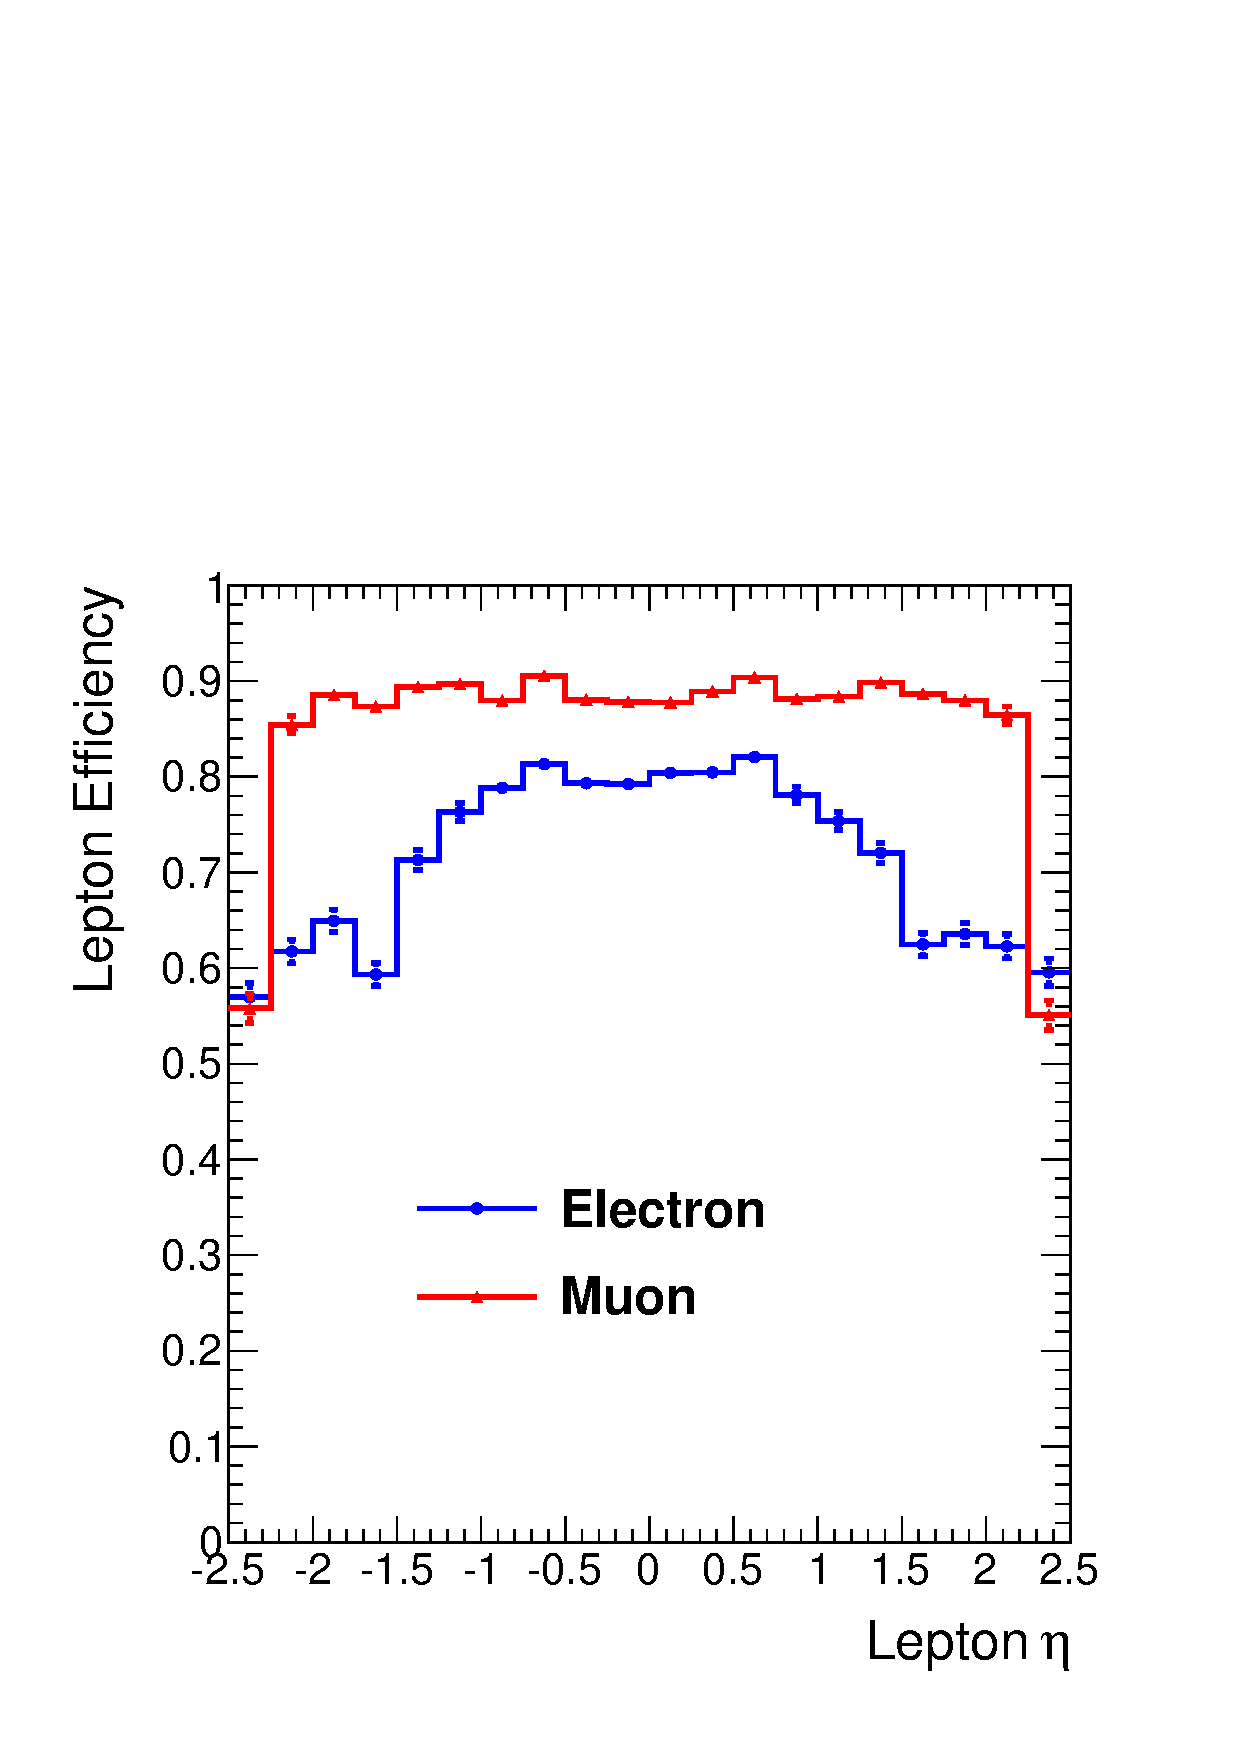
\includegraphics[width=0.4\textwidth]{figures/lepton_eff_Eta.pdf}
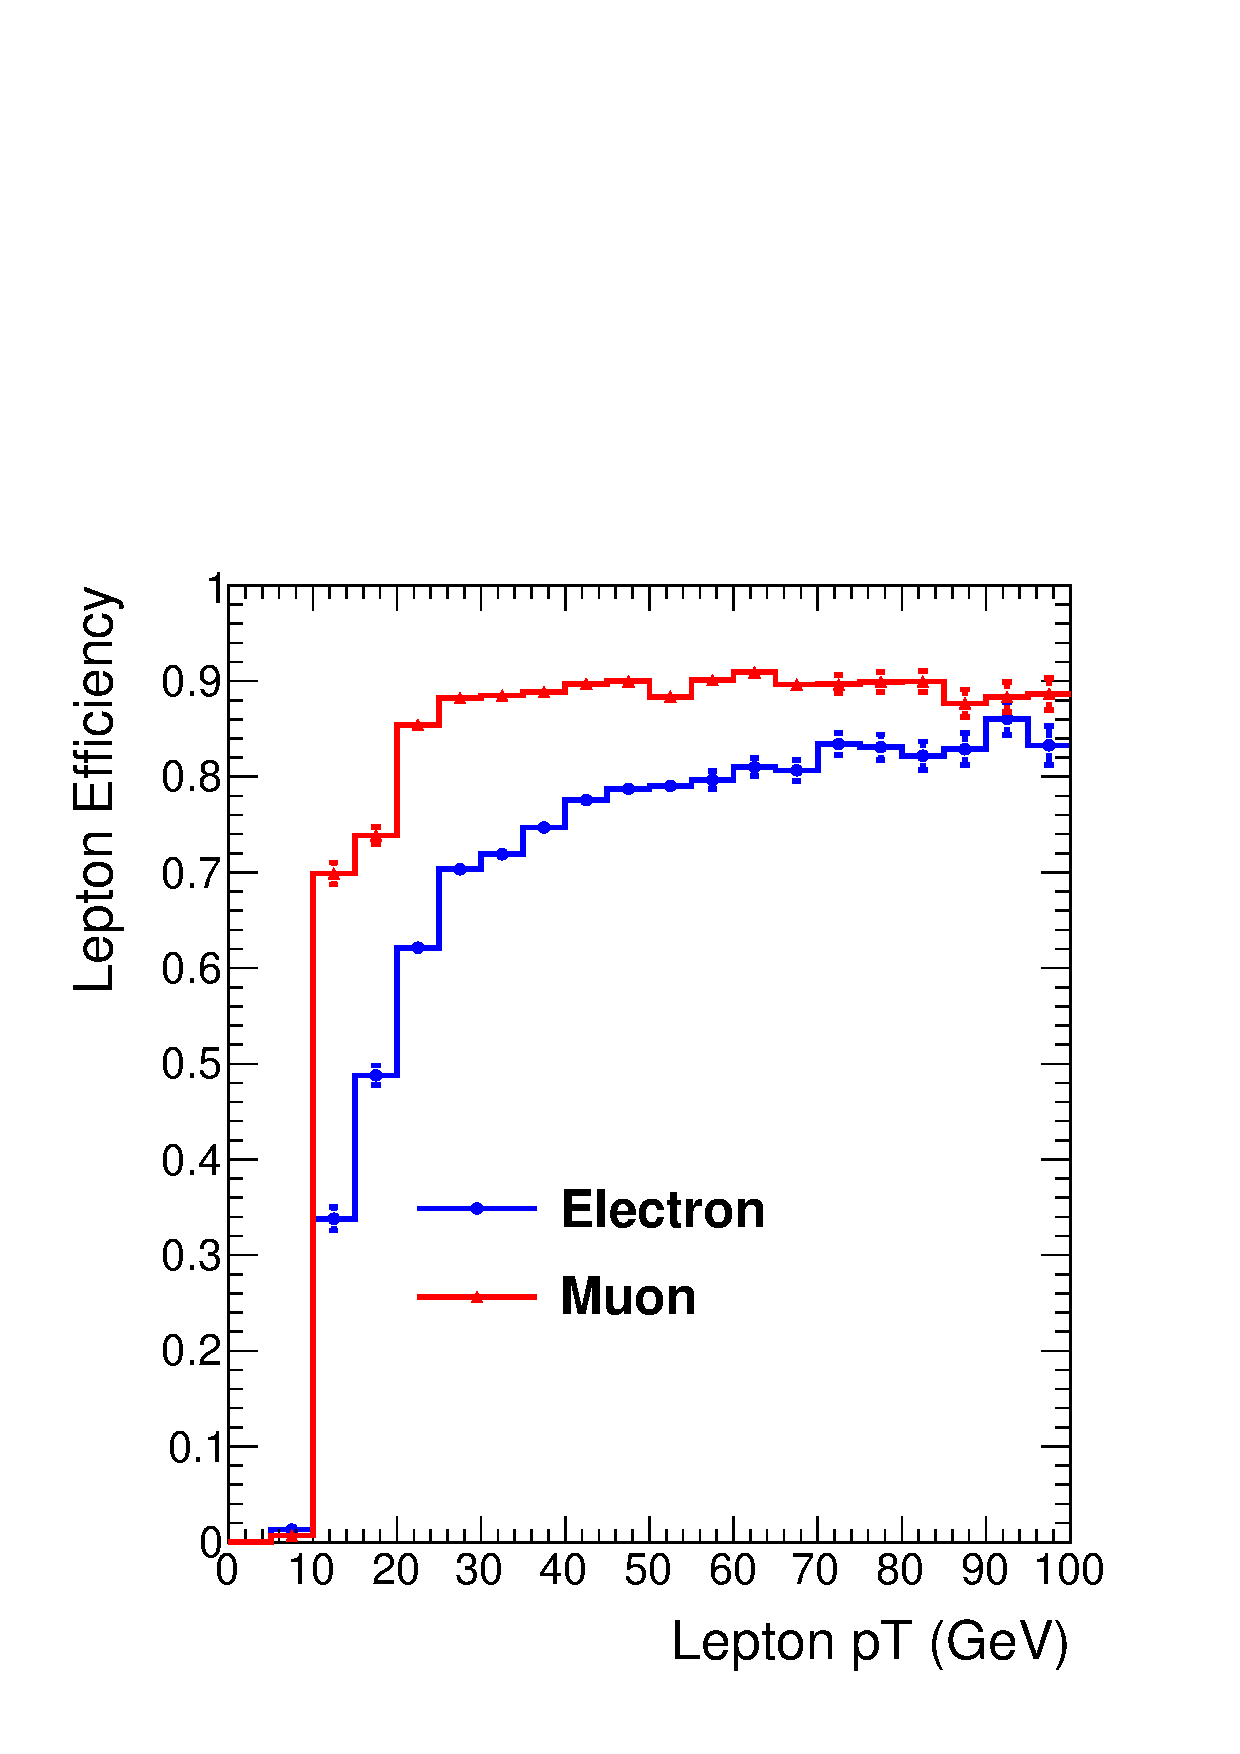
\includegraphics[width=0.4\textwidth]{figures/lepton_eff_Pt.pdf}\\
\caption{Lepton efficiency as a function of the lepton $\eta$ (left) and $p_{T}$ (right) extracted 
from the $WW$ Monte Carlo.}
\label{fig:lepeff_gen}
\end{center}
\end{figure}

Transfer functions $G(x;y)$ provide the probability of measuring the set of reconstructed variables ($x$) originating 
from a set of production variables ($y$). 
The general idea of these functions is to introduce a relation between the kinematic properties of parton-level objects
and reconstructed objects.
The set ($y$) represents the final state charged lepton and neutrino momenta at
the particle level, while the set ($x$) represents the measured lepton momenta and $\met$ in the CMS
detector. 
In the case of well-measured objects, such as lepton momenta, it is assumed that the reconstructed quantity is equal
to the generator level quantity.  The transfer function $G(x;y)$ is then considered to be a $\delta$-function, and the 
reconstructed lepton momenta are used in the differential cross-section calculations. For unmeasured quantities, such as
the longitudinal component of the neutrino momenta, the transfer function is unity. The sum of the transverse components
of the neutrino momenta can be inferred from energy and momentum conservation.

\subsubsection{Fake Leptons}
\label{sec:FakeLeptons}
The determination of the event probability for $W$+jet events must be handled slightly differently from other processes.
For these events to be reconstructed in the dilepton final state, one of the identified reconstructed leptons has been
faked by a parton fragmenting and hadronizing into a QCD jet which then fakes the signature of a lepton in the detector. 
To account for this effect properly, we multiply the differential cross-section for the $W$+jet process by the 
probability for a parton to be reconstructed as a lepton with the measured kinematics. This probability can be 
factorized into two terms:
\begin{eqnarray}
\begin{array}{lcl}
P(parton\rightarrow lepton)=P(parton\rightarrow FO) \times P(FO\rightarrow lepton),
\end{array} 
\end{eqnarray} 
where FO refers to a so-called ``fakeable object''. The first term in the product is measured using Monte Carlo and 
parametrized in $p_{T}$ and $\eta$. The second term is the fake rate measured in the data. The values 
of $P(parton \rightarrow lepton)$ are illustrated in Figure~\ref{fig:lepgenfr} for electrons and muons.
In both cases, $P$ is in the range $10^{-3}-10^{-4}$.

We cross check $P(parton \rightarrow lepton)$ values that we obtain using this method by comparing them to values 
measured in a $\gamma$+jet Monte Carlo and data samples.  In Monte Carlo, we check that in both samples, $W$+jet and  $\gamma$+jet,
electron fakeable objects originate most frequently from light quarks while muon fakeable objects are coming primarily
from semi-leptonic decays of charm and bottom quarks, as shown in Figure~\ref{fig:fakeorigins}.
Then using  $\gamma$+jet events we calculate the probability as ratio of the number of fakeable objects and number of jets in each $\eta$ and $p_{T}$ bin.
Probabilities obtained using these two methods agree well within the uncertainty. 

It should be also noted that in most cases the momentum of a fake lepton is significantly smaller than that of the faking parton.
To account for this effect we use the transfer function to map the parton-level quark or gluon momentum to the reconstructed
momentum of the fake lepton.
We extract this function from Monte Carlo by matching status code 3 partons to fakeable objects within a
cone of $\Delta R=0.2$.
The function is parametrized in the $p_{T}$ of the fakeable object and is shown in Figure~\ref{fig:ptresponse}.
In principle, not only $p_{T}$ but also the direction of the parton can differ from the reconstructed direction of the fakeable object.
However, we find that in the vast majority of cases they lie within $\Delta R<0.1$, as shown in Figure~\ref{fig:partonleptondirection},
and the difference has very little effect on the results of the analysis. Therefore, we do not apply any corrections to the direction
of the parton.


\begin{figure}[!htbp]                                                                                         
\begin{center}                                                                                                
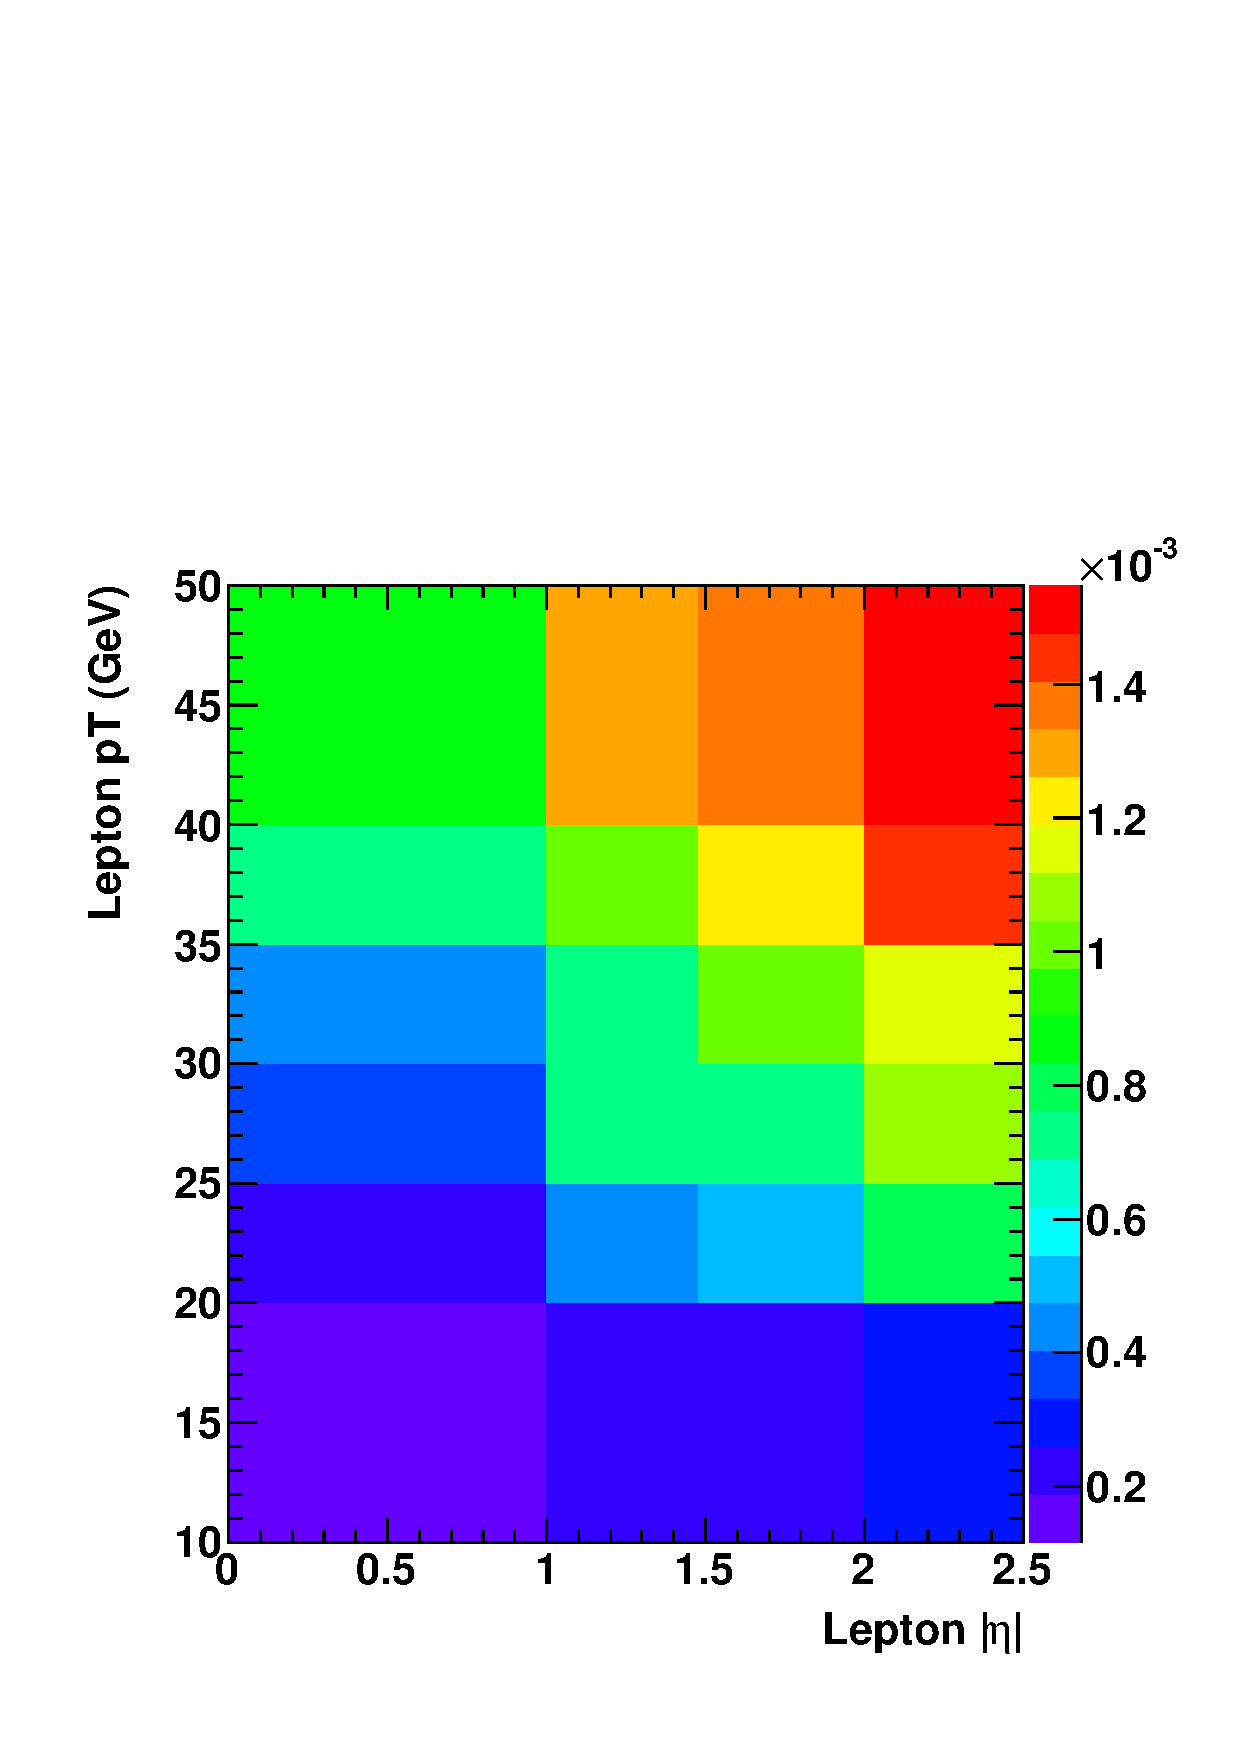
\includegraphics[width=0.4\textwidth]{figures/wjets_heleGenFR.pdf}                                            
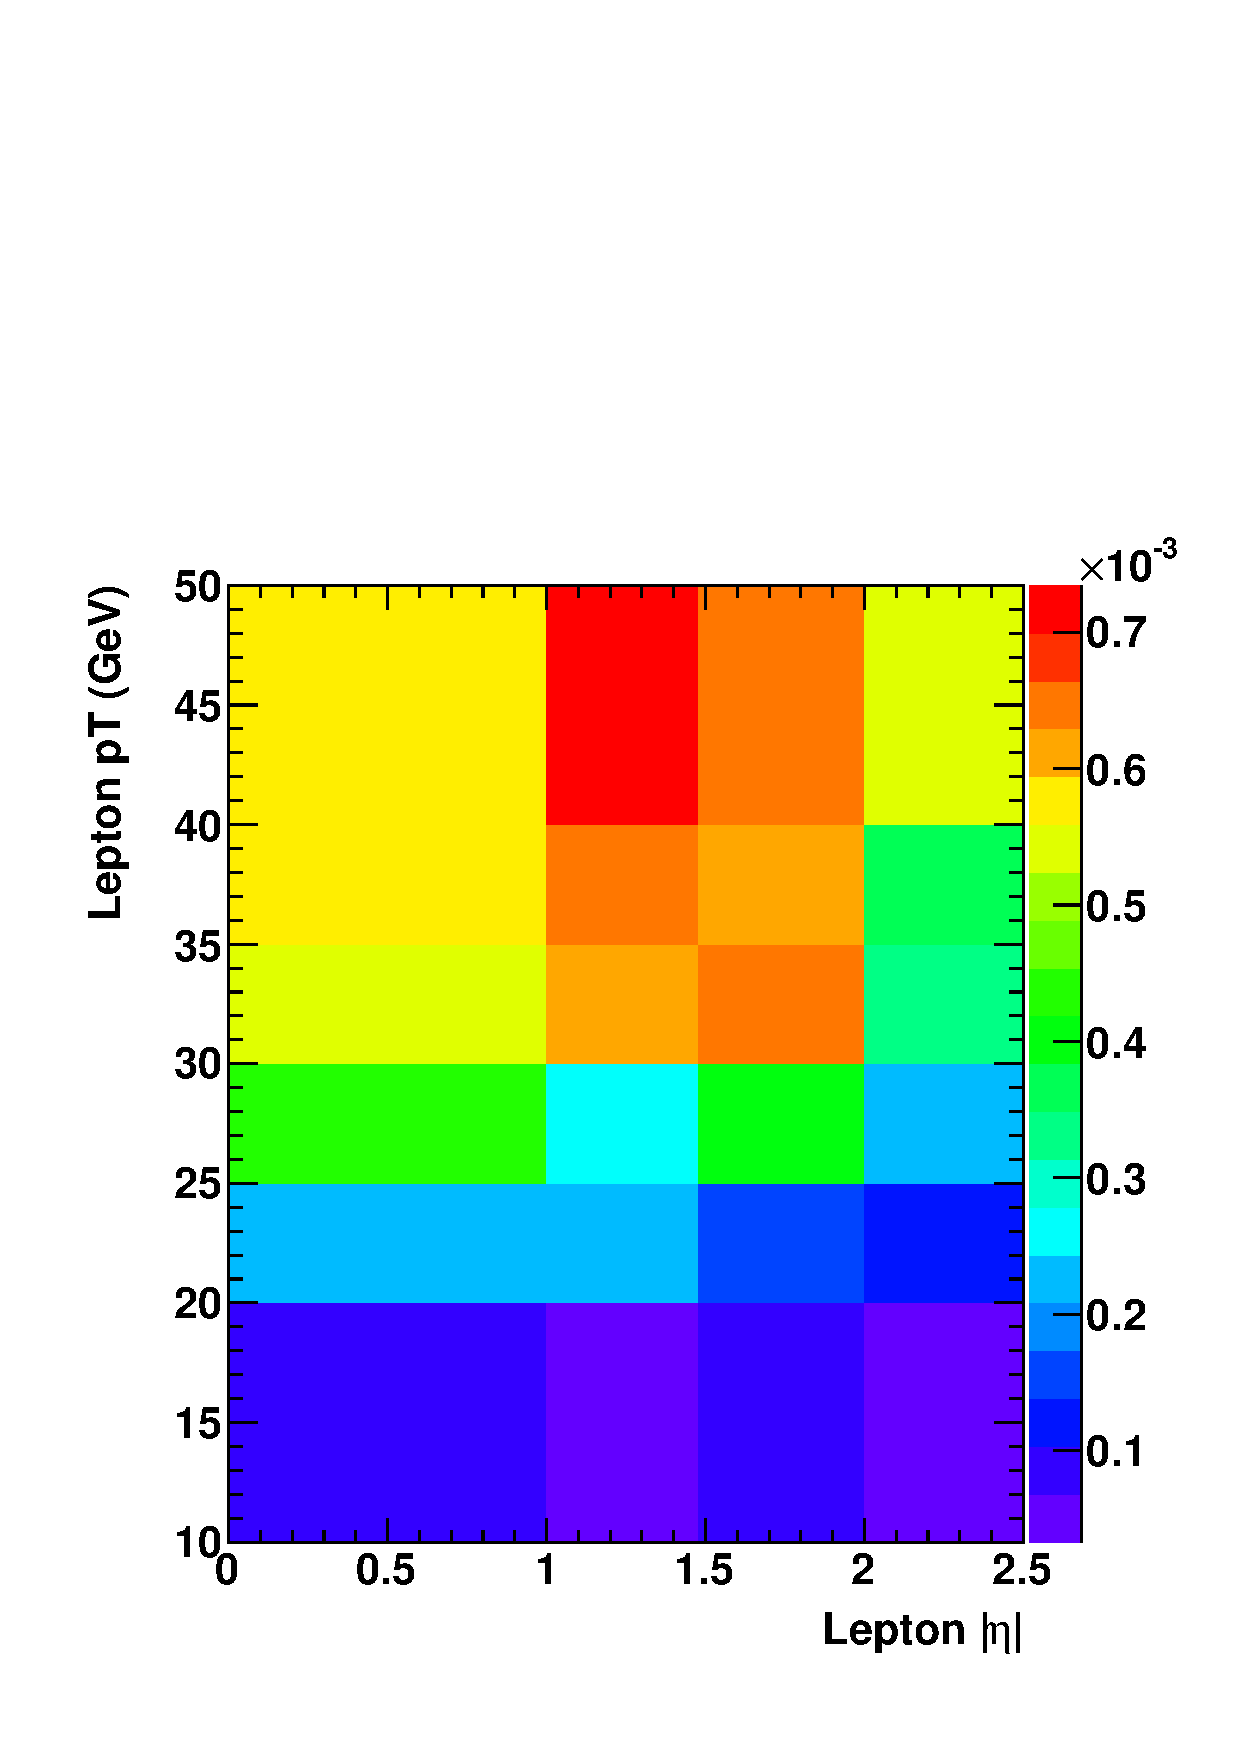
\includegraphics[width=0.4\textwidth]{figures/wjets_hmuGenFR.pdf}\\                                           
\caption{The probability for a parton to pass the electron (left) and muon (right)                            
fakeable object selections. }                                                                                 
\label{fig:lepgenfr}                                                                                          
\end{center}                                                                                                  
\end{figure}   

\begin{figure}[!htbp]                                                                                         
\begin{center}                                                                                                
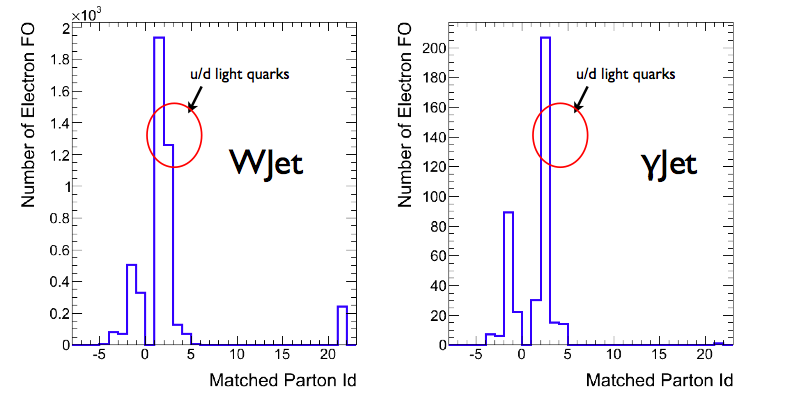
\includegraphics[width=0.9\textwidth]{figures/ElectronFakeOrigin.png}                                            
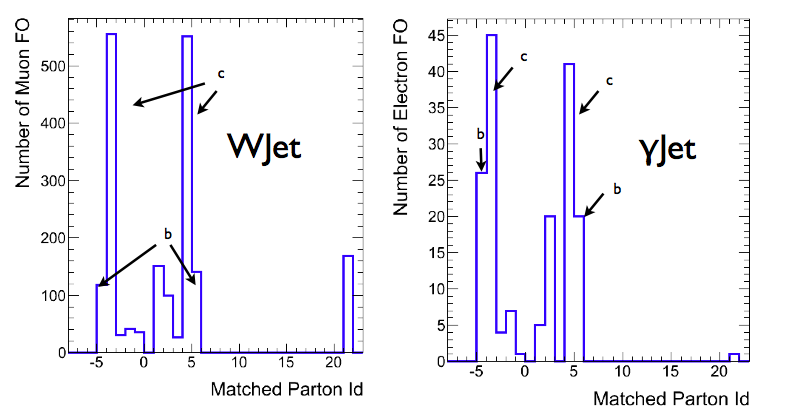
\includegraphics[width=0.9\textwidth]{figures/MuonFakeOrigin.png}\\                                           
\caption{ Origin of the electron and muon fakeable objects. The plot shows 
that electron fakes originate mostly from light quarks while muon fakes
are coming primarily from semi-leptonic heavy quark decays.}
\label{fig:fakeorigins}                                                                                          
\end{center}                                                                                                  
\end{figure}   


\begin{figure}[!htbp]                                                                                         
\begin{center}                                                                                                
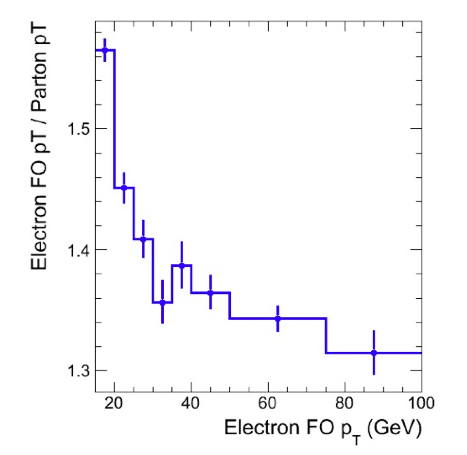
\includegraphics[width=0.4\textwidth]{figures/ElectronPtResponse.png}                                            
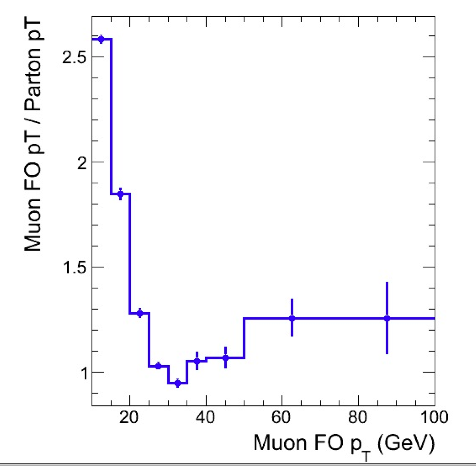
\includegraphics[width=0.4\textwidth]{figures/MuonPtResponse.png}\\                                           
\caption{Ratio of transverse momentum of a fakeable object and parton transverse momentum
for electron (left) and muons (right). }                                                                                 
\label{fig:ptresponse}                                                                                          
\end{center}                                                                                                  
\end{figure}   

\begin{figure}[!htbp]                                                                                         
\begin{center}                                                                                                
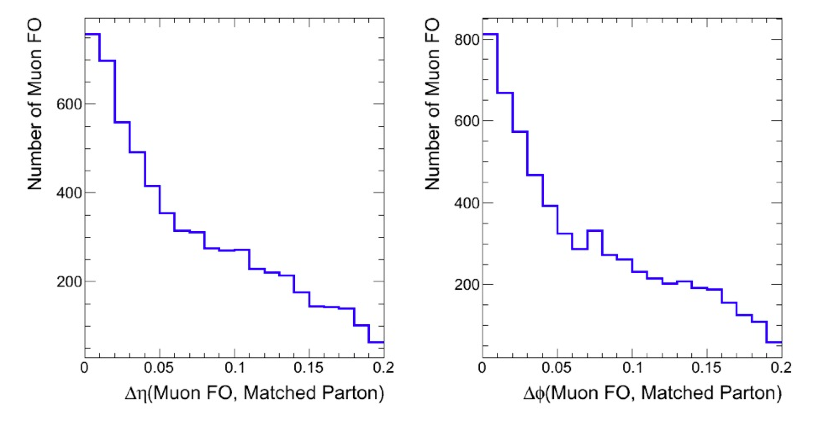
\includegraphics[width=0.8\textwidth]{figures/PartonLeptonDIrection.png}                                            
\caption{Distance in pseudo-rapidity (left) and azimuthal angle (right)
between generator level parton and reconstructed fakeable object.}                                                                                 
\label{fig:partonleptondirection}                                                                                          
\end{center}                                                                                                  
\end{figure}   


\clearpage
\subsubsection{Final Discriminant: Likelihood Ratio}
\label{sec:LR}
The Matrix Element functions used in this analysis are obtained from MCFM v5.8.  
MCFM provides both LO, and NLO cross-section calculations for 
all relevant background and Higgs production processes in $pp$ collisions. In this analysis 
we use only the LO Matrix Element. In the future we plan to improve our discriminant 
by taking advantage of the NLO Matrix Element. The PDF set used in the event probability 
calculations is CTEQ 6.1M.

Construction of the most optimal discriminant would require calculation 
of event probabilities for each of the background processes. In reality, however, having 
probabilities for only the signal hypothesis and the primary backgrounds is sufficient to achieve 
the desired level of discrimination. In this analysis we calculate for each event the probabilities 
for gluon fusion Higgs boson production (ggH), non-resonant $q\bar{q}\rightarrow WW$ pair 
production (WW) and the $W$+jet process where a $W$ boson is produced in association
with one jet.   For ggH we calculate the event probability given a specific hypothesis for the
mass and width of the Higgs.

Event probabilities, calculated as described above, are used to construct 
a likelihood ratio (LR) discriminant, which we use in a one-dimensional template fit.  
The discriminator is defined as :
\begin{equation}
\label{eqn:LR}
LR = \frac { P_s} { P_s + \sum_i k_{bi} P_{bi}},
\end{equation}
where $P_s$ is the signal probability, $P_{bi}$ is the probability of background $i$, and 
 $k_{bi}$ is the relative ratio of expected contribution of each background after the pre-selection, satisfying $\sum k_{bi} =1$.
In our particular case of two background process hypothesis, Eq.~\ref{eqn:LR} reduces to:
\begin{equation}
\label{eqn:LRHWW}
LR = \frac { P_{HWW}} { P_{HWW} + k_{WW} P_{WW}+k_{W+jet} P_{W+jet}},
\end{equation}
The calculation of $P_{HWW}$ is a function of Higgs mass so that the likelihood ratio
shape depends on $m_H$. This is true for both signal and background templates of $LR$.

It is important to note that because the LR distribution is calculated the same way for data,
signal MC, and background MC, the fact that we use the LO Matrix Element and make certain 
approximations in the analytic calculation may result in less than optimal sensitivity, but
it does not introduce any biases.
